\documentclass{article}
%% Useful packages
\usepackage[utf8]{inputenc}
\usepackage{float}
\usepackage[final]{graphicx}
\usepackage[a4paper,left=2cm,right=2cm,top=2cm,bottom=2cm]{geometry}
\usepackage{crop,graphicx,amsmath,array,color,amssymb,fancyhdr,lineno}
\usepackage{flushend,stfloats,amsthm,chngpage,times,,lipsum,lastpage}
\usepackage{calc,listings,color,wrapfig,tabularx,longtable,enumitem}
\usepackage[style=numeric-comp,backend=biber]{biblatex}
\usepackage[utf8]{inputenc}
\usepackage{pgfplots}
\usepackage{multicol}
\pgfplotsset{width=10cm,compat=1.9}
\usepgfplotslibrary{external}
\usepgfplotslibrary{dateplot}
\tikzexternalize
\addbibresource{Refs.bib}
\usepackage{lineno}
%%%%%%%%%%%%   Header and Footer  %%%%%%%%%%%%%
\pagestyle{fancy}
\fancypagestyle{plain}{%
  \renewcommand{\headrulewidth}{0pt}%
  \fancyhf{}%
}

\title{%
  Lab 1\\
  \large Cluster Benchmarking using EC2 Virtual Machines and Elastic Load Balancer (ELB)}
\author{Random Name}

\begin{document}
\begin{titlepage}

\newcommand{\HRule}{\rule{\linewidth}{0.5mm}} % Defines a new command for the horizontal lines, change thickness here

%----------------------------------------------------------------------------------------
%	LOGO SECTION
%----------------------------------------------------------------------------------------
\center

\includegraphics[width=10cm]{Title/polytechnique.png}\\[1cm] % Include a department/university logo - this will require the graphicx package
 
%----------------------------------------------------------------------------------------

\center % Center everything on the page

%----------------------------------------------------------------------------------------
%	HEADING SECTIONS
%----------------------------------------------------------------------------------------

\textsc{\LARGE Polytechnique Montréal }\\[1.5cm] % Name of your university/college
\textsc{\Large LOG8415E}\\[0.5cm] % Major heading such as course name
\textsc{\large Advanced Concepts of Cloud Computing}\\[0.5cm] % Minor heading such as course title

%----------------------------------------------------------------------------------------
%	TITLE SECTION
%----------------------------------------------------------------------------------------
\makeatletter
\HRule \\[0.4cm]
{ \huge \bfseries \@title}\\[0.4cm] % Title of your document
\HRule \\[1.5cm]
 
%----------------------------------------------------------------------------------------
%	AUTHOR SECTION
%----------------------------------------------------------------------------------------

\begin{minipage}{0.4\textwidth}
\begin{flushleft} \large
\emph{Authors:}\\
2009913 - Jordan Mimeault\\
2018968 - Antoine Lombardo\\
2020511 - Jacob Dupuis\\
2024785 - Alexandre Dufort\\[1.2em]
\end{flushleft}
\end{minipage}
~
\begin{minipage}{0.4\textwidth}
\begin{flushright} \large
\emph{Lab Instructor:} \\
Vahid Majdinasab  \\[1.2em] % Supervisor's Name
\emph{Instructor:} \\
Amin Nikanjam % second marker's name
\end{flushright}
\end{minipage}\\[2cm]
\makeatother

% If you don't want a supervisor, uncomment the two lines below and remove the section above
%\Large \emph{Author:}\\
%John \textsc{Smith}\\[3cm] % Your name

%----------------------------------------------------------------------------------------
%	DATE SECTION
%----------------------------------------------------------------------------------------

{\large October 17, 2022}\\[2cm] % Date, change the \today to a set date if you want to be precise

\vfill % Fill the rest of the page with whitespace

\end{titlepage}

\sffamily

\fancyhf{}
\fancyhead[L]{LOG8415E}
\fancyhead[R]{Lab 1}
\fancyfoot[R]{ \bf\thepage\ \rm }%

\newpage
\tableofcontents

\newpage
\section{Flask Application Deployment Procedure} \label{T1}

\paragraph{}The deployment of our application can be done using the first option of our run.sh script. This script guides the user while configuring AWS, then run a Python script that uses Boto3 for creating Security Groups, Instances, Target Groups and Load Balancer. Boto 3 is a AWS SDK that can be used to create, configure, and manage AWS services. That script will automatically flush old instances and other configurations then configure everything correctly to make sure everything always work as expected.
\paragraph{}The deployment of the Flask application in every instances is done with the use of a user\_data script, which allows us to perform automated configuration tasks and run the Flask app instance starts. Our user\_data script first installs git on each instance, then clone our git repository. It then install all the Python requirements then run the Flaks app on the instance. After that, each instance starts to respond to the port 80.
\paragraph{}To make sure that our Flask app keeps running, we used nohup, which instructs the system to continue running it even if the session is disconnected. That way, we can be sure that the Flask app we started won't stop.
\section{Cluster setup using Application Load Balancer.} \label{T2}

\paragraph{}We created two clusters (target groups) named cluster1 and cluster2. cluster1 targets every t2 instances, while cluster2 targets every m4 instances. These target groups allows us to redirect traffic to the desired type of instance, depending on the rules specified in the Load Balancer.
\paragraph{}For the Load Balancer, we created an internet-facing Application Load Balancer. We then added a Listener that listens to the HTTP port 80. We specified rules to redirect traffic to the correct clusters, depending on the path that needs to be accessed. The first rule forwards the request to cluster1 if the path is /cluster1, the second rule forwards the request to cluster2 if the path is /cluster2, and the default route returns a fixed response which is a 404 NOT FOUND error, indicating that the routes leads to no specified cluster.


\pagebreak
\section{Benchmark results} \label{T3}
\paragraph{} We performed several measurements on the load balancer, cluster 1 (t2.large instances) and cluster 2 (m4.large instances). We have 6 diagrams representing all interesting data for the comparison of the 2 clusters. First, we calculated the number of requests made over a time interval. We did this for the load balancer as well as for the two clusters. Then, we have 3 diagrams representing the status codes, i.e. all the codes 2XX, 4XX and 5XX of the requests sent previously. Finally, the last diagram represents the average response time of each cluster for the same requests of diagram 1.

\paragraph{} All the data was fetch using Boto3 CloudWatch API. Our script was made to automatically generate latex plots.


\begin{center}
    \textbf{Requests count for the load balancer}\break
    \begin{tikzpicture}
        \begin{axis}[
            date coordinates in=x,
            xticklabel=\hour:\minute,
            ymin=0,
            xlabel=Time,
            ylabel=RequestCount
            ]
            
            \addplot coordinates {
                (10-17-2022 21:20, 0.0)
                (10-17-2022 21:21, 862.0)
                (10-17-2022 21:22, 638.0)
                (10-17-2022 21:23, 1699.0)
                (10-17-2022 21:24, 801.0)
                (10-17-2022 21:25, 1000.0)
                (10-17-2022 21:26, 0.0)
                (10-17-2022 21:27, 0.0)
                (10-17-2022 21:28, 0.0)
                (10-17-2022 21:29, 0.0)
                (10-17-2022 21:30, 0.0)
            };
            \legend{
                Load Balancer
            }
        \end{axis}
    \end{tikzpicture}\\
    \emph{Figure 3.1 - Requests count for the load balancer}
\end{center}
\paragraph{} As we can see in the graph above (figure 3.1), the requests count of the load balancer totals around 5000 requests, which was expected since it includes all requests made to both clusters.\\

\begin{center}
    \textbf{Requests count for cluster1 and cluster2}\break
    \begin{tikzpicture}
        \begin{axis}[
            date coordinates in=x,
            xticklabel=\hour:\minute,
            ymin=0,
            xlabel=Time,
            ylabel=RequestCount
        ]
            \addplot coordinates {
                (10-17-2022 21:20, 0.0)
                (10-17-2022 21:21, 862.0)
                (10-17-2022 21:22, 638.0)
                (10-17-2022 21:23, 1000.0)
                (10-17-2022 21:24, 0.0)
                (10-17-2022 21:25, 0.0)
                (10-17-2022 21:26, 0.0)
                (10-17-2022 21:27, 0.0)
                (10-17-2022 21:28, 0.0)
                (10-17-2022 21:29, 0.0)
                (10-17-2022 21:30, 0.0)
            };
            \addplot coordinates {
                (10-17-2022 21:20, 0.0)
                (10-17-2022 21:21, 0.0)
                (10-17-2022 21:22, 0.0)
                (10-17-2022 21:23, 699.0)
                (10-17-2022 21:24, 801.0)
                (10-17-2022 21:25, 1000.0)
                (10-17-2022 21:26, 0.0)
                (10-17-2022 21:27, 0.0)
                (10-17-2022 21:28, 0.0)
                (10-17-2022 21:29, 0.0)
                (10-17-2022 21:30, 0.0)
            };
            \legend{
                Cluster 1 (t2), Cluster 2 (m4)
            }
        \end{axis}
    \end{tikzpicture}\\
    \emph{Figure 3.2 - Requests count for cluster1 and cluster2}
\end{center}

\paragraph{} This diagram (figure 3.2) shows that each cluster treats the requests similarly because the request count is similar over the time. Both clusters received a total of 2500 requests, which is what we expected since we sent 2500 requests to each route. This means that the load balancing is done effectively for both t2 and m4 instances.\\


\begin{center}
    \textbf{HTTP code 2XX count}\break
    \begin{tikzpicture}
        \begin{axis}[
            date coordinates in=x,
            xticklabel=\hour:\minute,
            ymin=0,
            xlabel=Time,
            ylabel=HTTPCode\_Target\_2XX\_Count
        ]
    
            \addplot coordinates {
                (10-17-2022 21:20, 0.0)
                (10-17-2022 21:21, 862.0)
                (10-17-2022 21:22, 638.0)
                (10-17-2022 21:23, 1000.0)
                (10-17-2022 21:24, 0.0)
                (10-17-2022 21:25, 0.0)
                (10-17-2022 21:26, 0.0)
                (10-17-2022 21:27, 0.0)
                (10-17-2022 21:28, 0.0)
                (10-17-2022 21:29, 0.0)
                (10-17-2022 21:30, 0.0)
                };
            
            \addplot coordinates {
                (10-17-2022 21:20, 0.0)
                (10-17-2022 21:21, 0.0)
                (10-17-2022 21:22, 0.0)
                (10-17-2022 21:23, 699.0)
                (10-17-2022 21:24, 801.0)
                (10-17-2022 21:25, 1000.0)
                (10-17-2022 21:26, 0.0)
                (10-17-2022 21:27, 0.0)
                (10-17-2022 21:28, 0.0)
                (10-17-2022 21:29, 0.0)
                (10-17-2022 21:30, 0.0)
                };
            \legend{
                Cluster 1 (t2), Cluster 2 (m4)
            }
        \end{axis}
    \end{tikzpicture}\\
    \emph{Figure 3.3 - HTTP code 2XX count}
    \paragraph{} This diagram (figure 3.3) shows that there are as many HTTP status code 2XX as there are requests because the diagram is identical to the diagram of the requests count. This means that there were no errors in the load balancing. This affirmation is confirmed by analyzing the next two diagrams (figures 3.4 and 3.5).
\end{center}

\begin{multicols}{2}
    \begin{center}
        \textbf{HTTP code 4XX count}\break
        \begin{tikzpicture}[scale=0.75]
            \begin{axis}[
                date coordinates in=x,
                xticklabel=\hour:\minute,
                ymin=0,
                xlabel=Time,
                ylabel=HTTPCode\_Target\_4XX\_Count
                ]
            
                \addplot coordinates {
                    (10-17-2022 21:20, 0.0)
                    (10-17-2022 21:21, 0.0)
                    (10-17-2022 21:22, 0.0)
                    (10-17-2022 21:23, 0.0)
                    (10-17-2022 21:24, 0.0)
                    (10-17-2022 21:25, 0.0)
                    (10-17-2022 21:26, 0.0)
                    (10-17-2022 21:27, 0.0)
                    (10-17-2022 21:28, 0.0)
                    (10-17-2022 21:29, 0.0)
                    (10-17-2022 21:30, 0.0)
                    };
                
                \addplot coordinates {
                    (10-17-2022 21:20, 0.0)
                    (10-17-2022 21:21, 0.0)
                    (10-17-2022 21:22, 0.0)
                    (10-17-2022 21:23, 0.0)
                    (10-17-2022 21:24, 0.0)
                    (10-17-2022 21:25, 0.0)
                    (10-17-2022 21:26, 0.0)
                    (10-17-2022 21:27, 0.0)
                    (10-17-2022 21:28, 0.0)
                    (10-17-2022 21:29, 0.0)
                    (10-17-2022 21:30, 0.0)
                    };
                    
                \legend{
                    Cluster 1 (t2), Cluster 2 (m4)
                }
            \end{axis}
        \end{tikzpicture}\\
        \emph{Figure 3.4 - HTTP code 4XX count}
    \end{center}
    \columnbreak
    \begin{center}
        \textbf{HTTP code 5XX count}\break
        \begin{tikzpicture}[scale=0.75]
            \begin{axis}[
                date coordinates in=x,
                xticklabel=\hour:\minute,
                ymin=0,
                xlabel=Time,
                ylabel=HTTPCode\_Target\_5XX\_Count
                ]
            
                \addplot coordinates {
                    (10-17-2022 21:20, 0.0)
                    (10-17-2022 21:21, 0.0)
                    (10-17-2022 21:22, 0.0)
                    (10-17-2022 21:23, 0.0)
                    (10-17-2022 21:24, 0.0)
                    (10-17-2022 21:25, 0.0)
                    (10-17-2022 21:26, 0.0)
                    (10-17-2022 21:27, 0.0)
                    (10-17-2022 21:28, 0.0)
                    (10-17-2022 21:29, 0.0)
                    (10-17-2022 21:30, 0.0)
                };
                
                \addplot coordinates {
                    (10-17-2022 21:20, 0.0)
                    (10-17-2022 21:21, 0.0)
                    (10-17-2022 21:22, 0.0)
                    (10-17-2022 21:23, 0.0)
                    (10-17-2022 21:24, 0.0)
                    (10-17-2022 21:25, 0.0)
                    (10-17-2022 21:26, 0.0)
                    (10-17-2022 21:27, 0.0)
                    (10-17-2022 21:28, 0.0)
                    (10-17-2022 21:29, 0.0)
                    (10-17-2022 21:30, 0.0)
                };
                \legend{
                    Cluster 1 (t2), Cluster 2 (m4)
                }
            \end{axis}
        \end{tikzpicture}\\
        \emph{Figure 3.5 - HTTP code 5XX count}
    \end{center}
\end{multicols}
\paragraph{} In above diagrams (figures 3.4 and 3.5), we can see that no error codes 4xx or 5xx were given. That means that no error occurred in any request, which allows us to say that no error has happen while doing our benchmarks.
\pagebreak
\begin{center}
    \textbf{Target average response time}\break
    \begin{tikzpicture}
        \begin{axis}[
            date coordinates in=x,
            xticklabel=\hour:\minute,
            ymin=0,
            xlabel=Time,
            ylabel=TargetResponseTime (ms)
            ]

            \addplot coordinates {
                (10-17-2022 21:20, 0.0)
                (10-17-2022 21:21, 1.689)
                (10-17-2022 21:22, 1.76)
                (10-17-2022 21:23, 1.909)
                (10-17-2022 21:24, 0.0)
                (10-17-2022 21:25, 0.0)
                (10-17-2022 21:26, 0.0)
                (10-17-2022 21:27, 0.0)
                (10-17-2022 21:28, 0.0)
                (10-17-2022 21:29, 0.0)
                (10-17-2022 21:30, 0.0)
            };
        
            \addplot coordinates {
                (10-17-2022 21:20, 0.0)
                (10-17-2022 21:21, 0.0)
                (10-17-2022 21:22, 0.0)
                (10-17-2022 21:23, 1.717)
                (10-17-2022 21:24, 1.789)
                (10-17-2022 21:25, 1.741)
                (10-17-2022 21:26, 0.0)
                (10-17-2022 21:27, 0.0)
                (10-17-2022 21:28, 0.0)
                (10-17-2022 21:29, 0.0)
                (10-17-2022 21:30, 0.0)
            };
            \legend{
                Cluster 1 (t2), Cluster 2 (m4)
            }
        \end{axis}
    \end{tikzpicture}\\
    \emph{Figure 3.6 - Target average response time for each cluster}\\
\end{center}
\paragraph{} This diagram (figure 3.6) shows that the cluster 2 has a slightly better average time of response than the cluster 1. However, the difference is so small that we cannot conclude anything over this. Overall, both clusters seem to perform similarly.
\pagebreak
\section{Instructions to run the code.} \label{T4}

\paragraph{}The script needs to be run and should run correctly on any linux environment. However, it has only been tested on a Debian environment. The pre-requisite to run the script is to have git, pip3, python3, aws and docker installed. To make sure the script is executable, the command \verb|sudo chmod +x script.sh| must be executed. Our bash script can then be run as root with the command \verb|sudo .\script.sh|. Out git repository will then be automatically cloned and the \verb|run.sh| script will be executed, which will automatically install all the necessary Python libraries.

\paragraph{}Alternatively, the script can be run manually. To do so, the repository must be cloned using this command:\\\verb|git clone https://github.com/JordMim/LOG8415E.git|. The script will then be located in the directory \verb|LOG8415E/tp1|. The script must be set as executable using the command \verb|sudo chmod +x run.sh|, and can then be run using the command \verb|sudo ./run.sh|.

\paragraph{}When running the script, you'll be asked to setup AWS credentials. If this is your first time using the script, you'll have to do this setup. After that, this step can be omitted, as it will fetch the default credentials saved in AWS.\\

\begin{center}
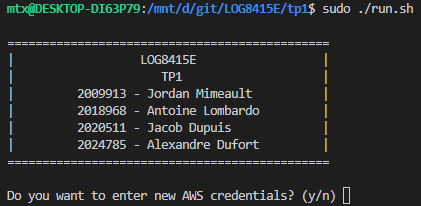
\includegraphics[width=10cm]{Resources/aws_credentials.png}\\
\emph{Figure 4.1 - Execution of command \verb|sudo ./run.sh|}
\end{center}\\

\paragraph{}When AWS configuration is done, you'll be asked what actions needs to be done. There are five options:
\begin{itemize}
  \item Configure AWS Load Balancer, which basically creates all the necessary AWS resources.
  \item Run requests sender, which runs the benchmark.
  \item Fetch metrics, which fetch CloudWatch metrics and export them into JSON and latex format.
  \item Only run benchmark and fetch metrics.
  \item Do everything.
\end{itemize}

\begin{center}
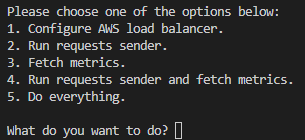
\includegraphics[width=8cm]{Resources/options.png}\\
\emph{Figure 4.2 - Possible options of action}
\end{center}\\

\lef\paragraph{}For each step of the script, the normal output should look like these:

\begin{center}\centering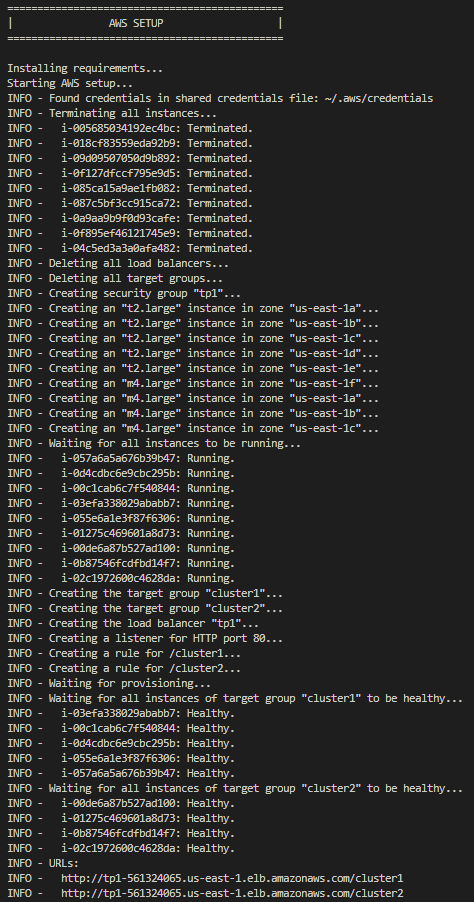
\includegraphics[width=10cm]{Resources/aws_setup.png}\\\emph{Figure 4.3 - Output of the AWS Setup step}\end{center}\\
\begin{center}\centering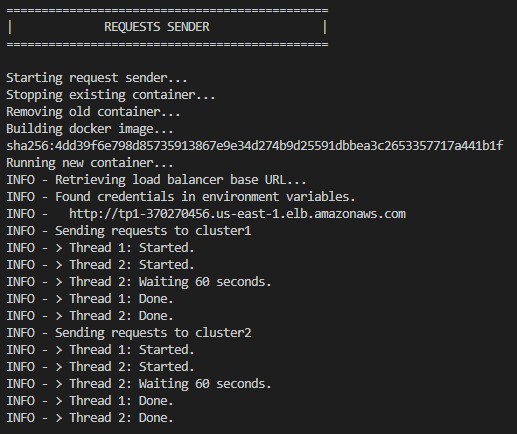
\includegraphics[width=10cm]{Resources/requests.png}\\\emph{Figure 4.4 - Output of the Requests Sender step}\end{center}\\
\begin{center}\centering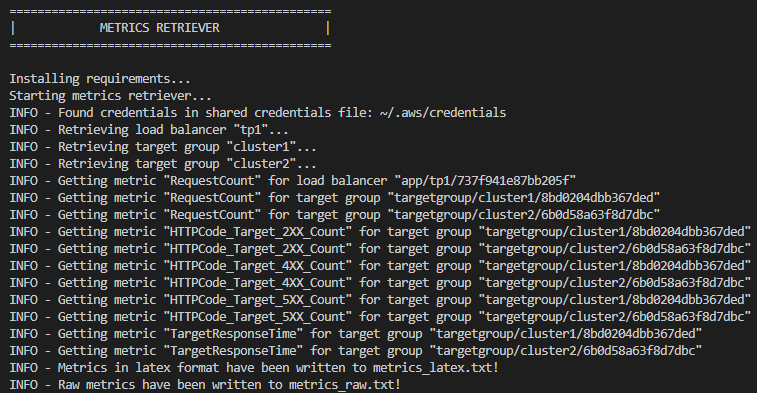
\includegraphics[width=10cm]{Resources/metrics.png}\\\emph{Figure 4.5 - Output of the Metrics Retriever step}\end{center}\\




\pagebreak
\printbibliography[heading=bibnumbered]


\end{document}
